%!TEX root=masterproef.tex

\subsection{Opbouw}

Figuur \ref{fig:devel-component-overview} geeft een overzicht van de opbouw van
de oplossing.

\begin{figure}[ht]
  \centering
  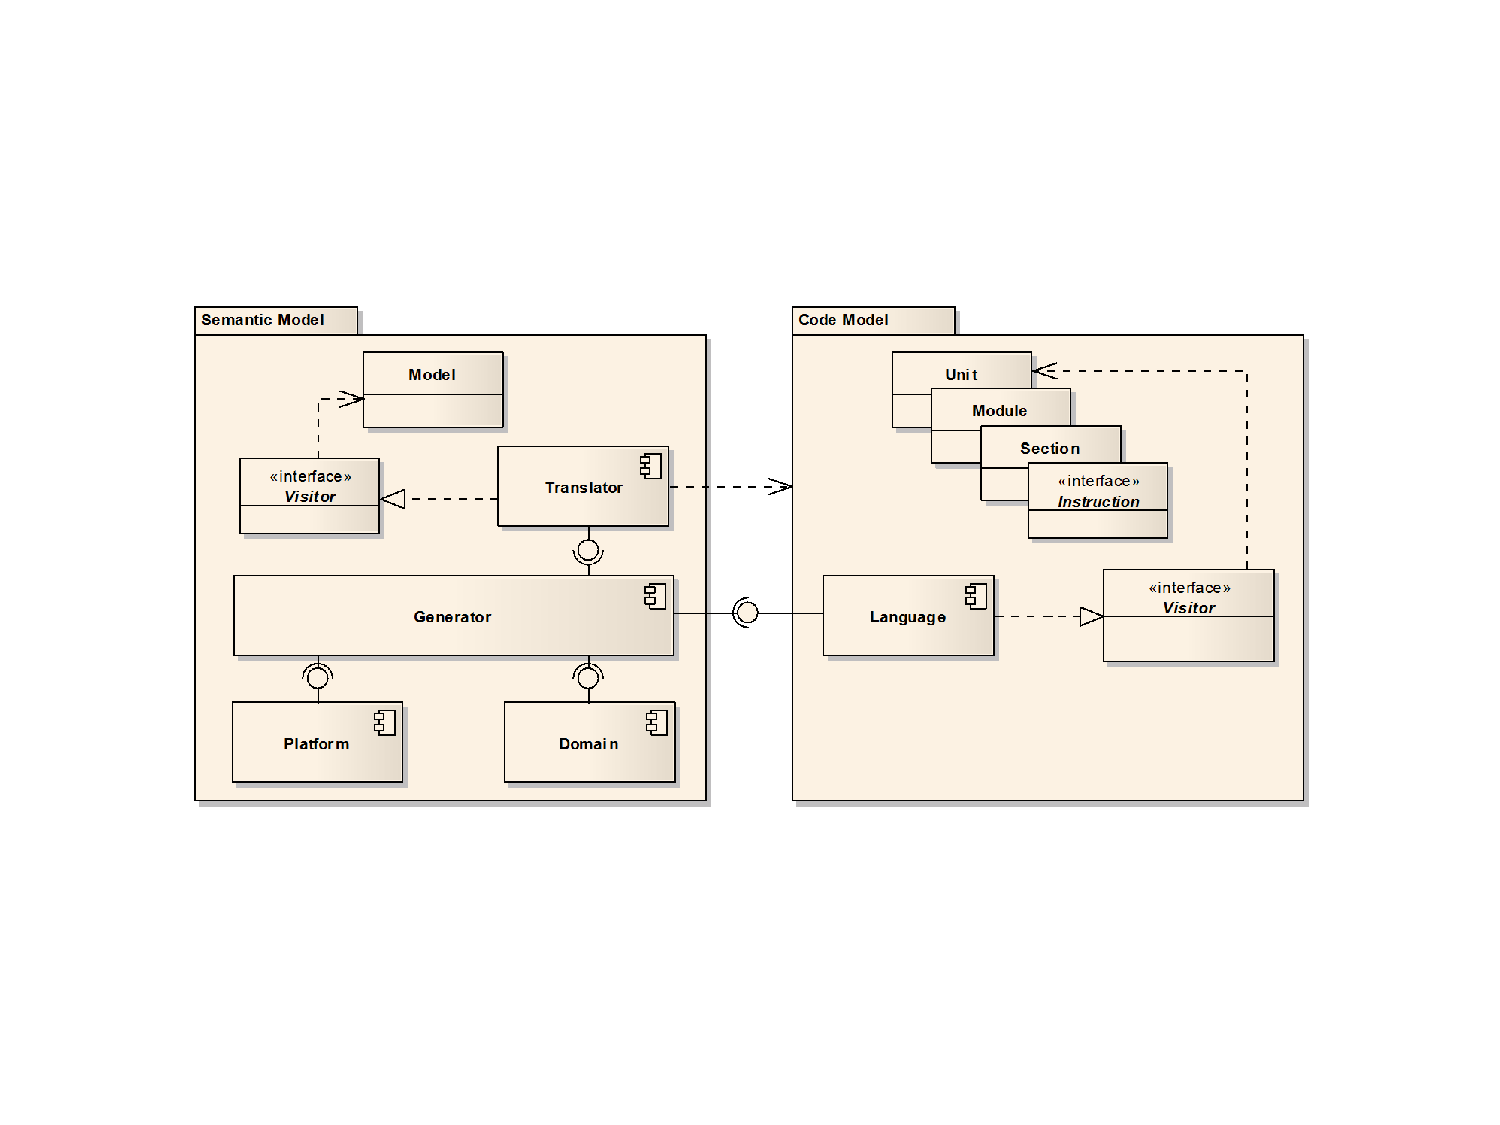
\includegraphics[width=\linewidth]{resources/component-overview.pdf}
  \caption{Overzicht van componenten en kernentiteiten}
  \label{fig:devel-component-overview}
\end{figure}

Intern bestaat de hele oplossing uit twee grote delen: het semantische en het
code gedeelte. Binnen het semantische gedeelte vinden we het SM terug. Dit
model kan benaderd worden door middel van een zgn. \emph{visitor}, een
implementatie van het \emph{visitor pattern}. Aan de hand van deze
\emph{visitor} kunnen transformaties van het model gerealiseerd worden.

Het SM is de primaire invoer voor de generator. Die kan zijn werk slechts
vervullen door middel van een compositie met \emph{platform-} en
\emph{domeininformatie}, een vertaler (\emph{Translator}) die elementen
uit het semantische gedeelte kan omzetten naar overeenkomstige elementen in het
code gedeelte en de uiteindelijk beoogde programmeertaal (\emph{Language}).

De programmeertaal maakt deel uit van het CM. Dit is op zijn beurt opgebouwd
uit een hi\"erarchie van vier niveaus. De structuur van de beoogde code wordt
weergegeven door de compilatie \emph{unit}, de \emph{modules} en de
\emph{secties}, waarbij de unit staat voor het geheel, de modules voor
functioneel samenhangende delen en de secties zorgen voor een fysieke opdeling
in bv. bestanden. De juiste realisatie van deze hi\"erarchie wordt overgelaten
aan de implementatie van de taal die hier betekenis kan aan geven.

Op het laagste niveau van het CM vinden we de \emph{instructies}. Deze kunnen
gebruikt worden om de effectieve code voor te stellen. Er bestaat in het CM per
definitie een overeenkomstige instructie voor elk element uit het SM. Aangezien
het SM functioneel rijker is dan de meeste programmeertalen, zal na constructie
van het initi\"ele CM, door middel van transformaties, alternatieven
ge\"implementeerd moeten worden binnen de mogelijkheden van de uiteindelijke
programmeertaal.

\subsection{ANTLR}
\label{subsection:devel-antlr}

Maar alles begint bij het inladen van de FOO-lang bronbestanden in het SM. Dit
gebeurt door middel van een \emph{parser} die de tekstuele voorstelling
analyseert en de taal-eigen constructies er uit puurt. Het resultaat van deze
stap is de constructie van een boomstructuur die de juiste semantische
betekenis van de verschillende constructie structureel weergeeft. Zo'n
boomstructuur is een AST. Figuur \ref{fig:devel-ast} toont de AST van het
elementaire voorbeeld uit codevoorbeeld \ref{lst:hello.foo}.

\begin{figure}[ht]
  \centering
  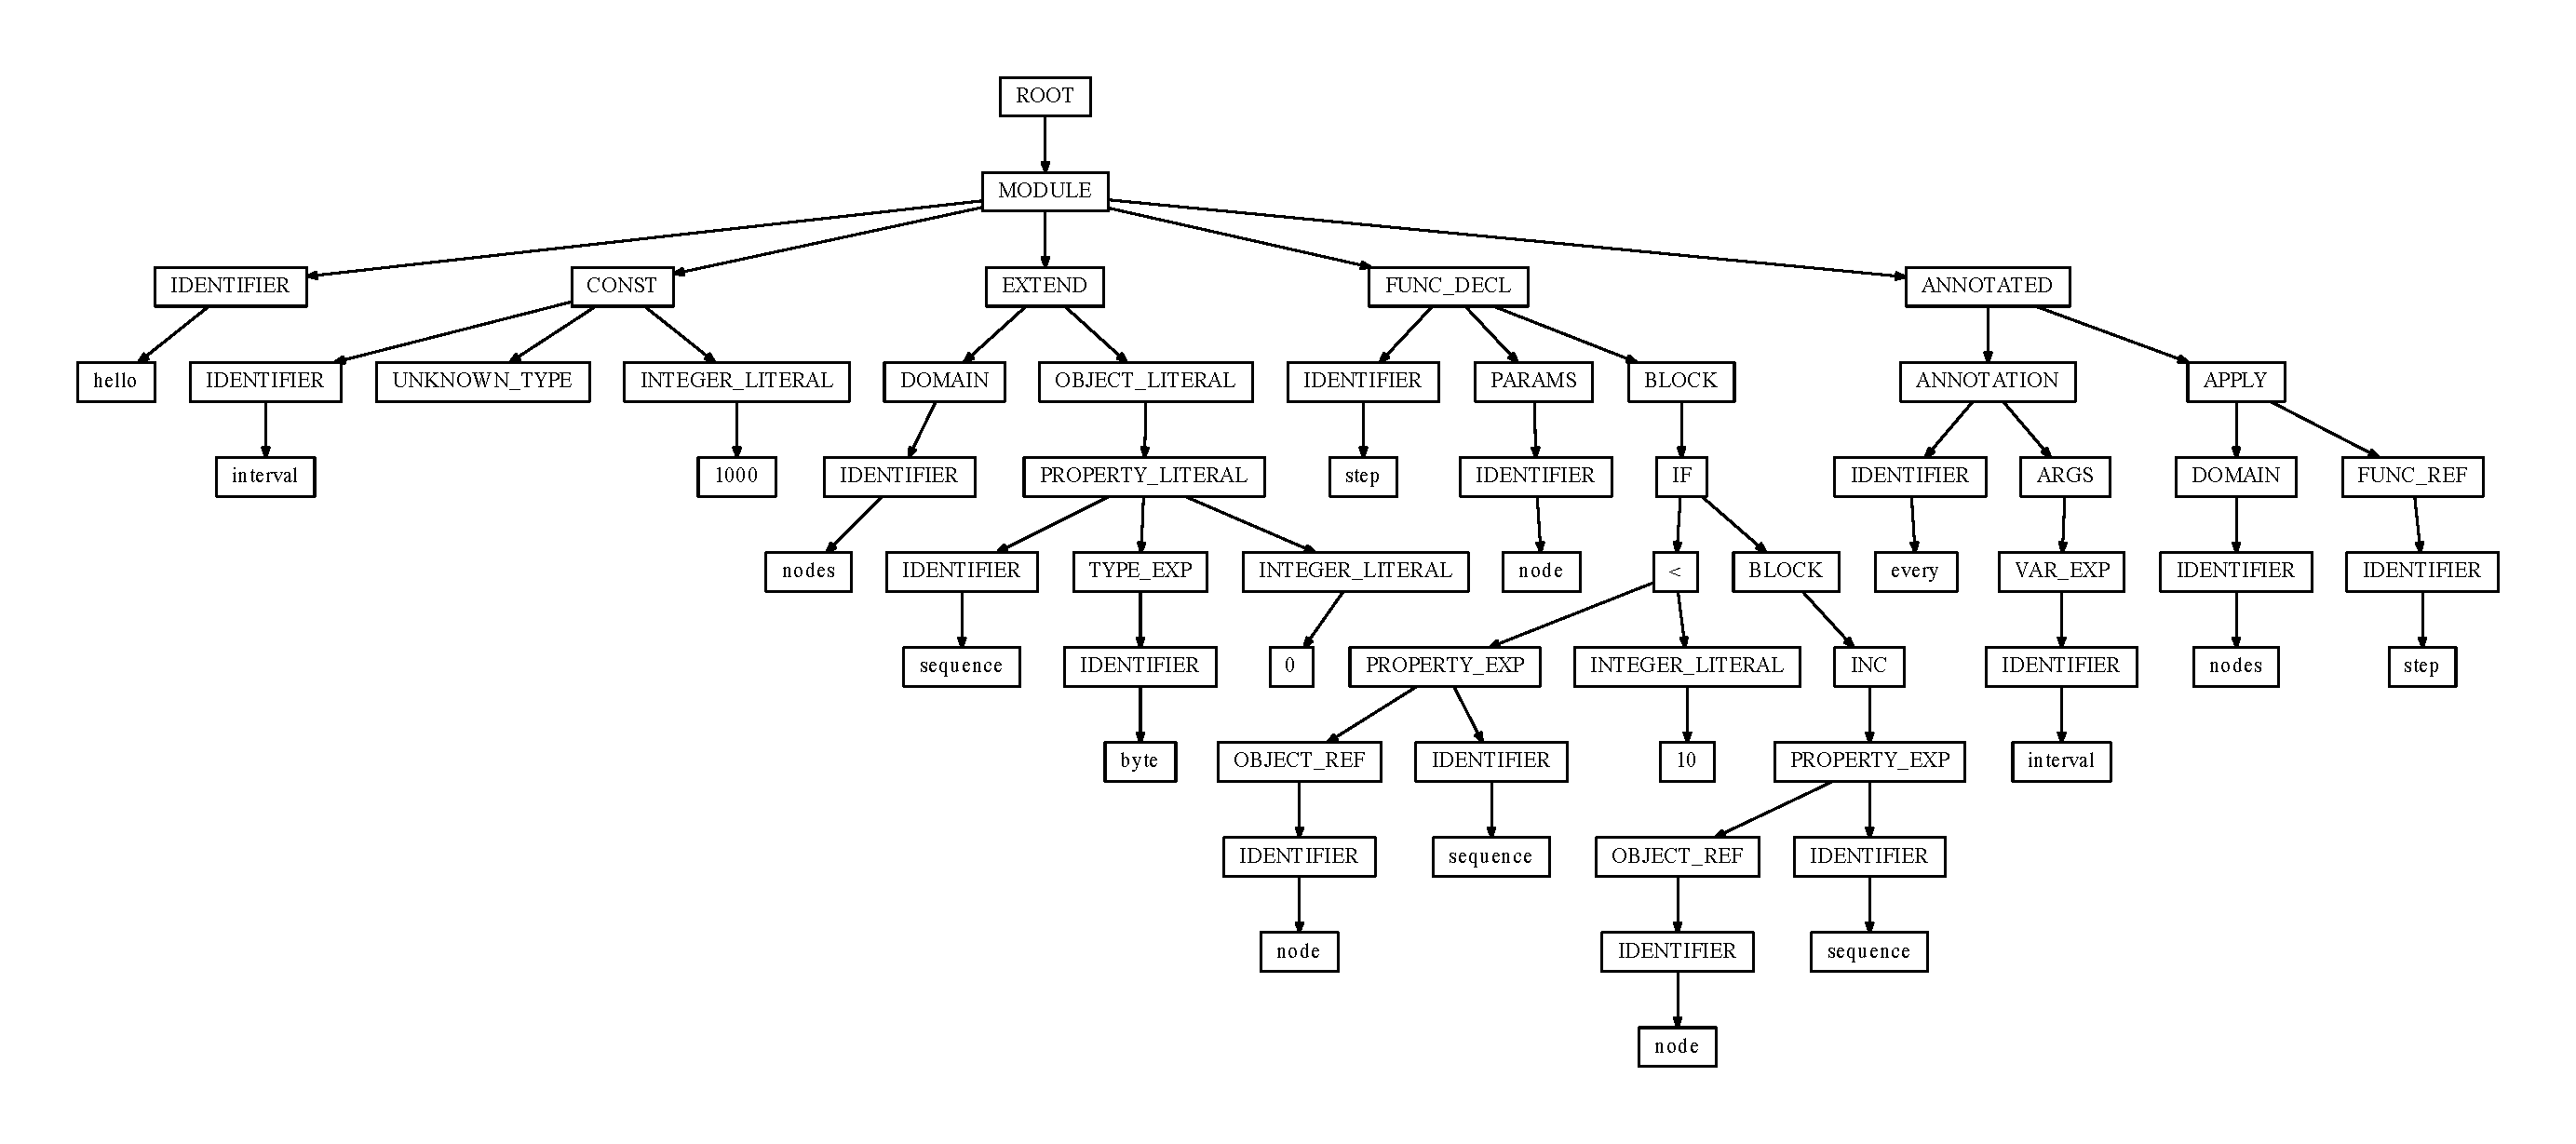
\includegraphics[width=\linewidth]{resources/hello_ast.pdf}
  \caption{De AST van het elementaire voorbeeld, \ttt{hello.foo}}
  \label{fig:devel-ast}
\end{figure}

We herkennen duidelijk de inhoud van het codevoorbeeld: op het hoogste niveau
zien we de module met een naam, de definitie van een constante, een uitbreiding
van het domein, een functie definitie en een geannoteerde applicatie van een
functie op een domein. De AST is ontdaan van alle ondersteunende syntax zoals
aanduidingen voor blokken code\dots en bevat louter de semantische inhoud.
